\documentclass[a4paper,12pt,ngerman]{article}

% Pakete
\usepackage[utf8]{inputenc}
\usepackage[T1]{fontenc}
\usepackage{babel} % Deutsche Sprache
\usepackage{csquotes} % Stellt korrekte Zitatformatierung bereit
\usepackage{cleveref}
\usepackage{geometry} % Seitenränder anpassen
\geometry{a4paper, left=3cm, right=3cm, top=3cm, bottom=3cm}
\usepackage{graphicx}

\usepackage{minted}
% \usemintedstyle{one-dark}  % Alternativer Farbstil

\usepackage[backend=biber,style=numeric,sorting=none]{biblatex}
%\bibliographystyle{plain}
\addbibresource{literature.bib}

\usepackage[ngerman,colorinlistoftodos]{todonotes}
\setlength{\marginparwidth}{2cm} % um die ToDo-Notes schöner am Seitenrand anzeigen zu lassen

\begin{document}
	
	% Deckblatt
	\begin{titlepage}
		\centering
		\vspace*{1cm}
		
		{\LARGE \textbf{Health Checker}}\\[1cm]
		
		{\large Projektdokumentation}\\[1.0cm]
		{\large Studiengang Systems Engineering (B.~Eng.)}\\[0.3cm]
		{\large Schwerpunkt I.2}\\[1.5cm]
		
		\vfill
    
		\textbf{Verfasser/innen:}\\[1cm]
    	\begin{center}
		\begin{minipage}[t]{0.45\textwidth}
        \raggedright
        Jan-Niclas Fenger \\
        Matrikelnummer: 2092175 \\
        E-Mail: jan-niclas.fenger@tha.de \\[0.5cm]
		
        Simon Schneider \\
        Matrikelnummer: 2151357 \\
        E-Mail: simon.schneider1@tha.de
		\end{minipage}
		\hfill
		\begin{minipage}[t]{0.45\textwidth}
        \raggedright
        Leopold Weber \\
        Matrikelnummer: 2155780 \\
        E-Mail: leopold.weber@tha.de \\[0.5cm]
    
        Janis Preiß \\
        Matrikelnummer: 2150826 \\
        E-Mail: janis.preiss@tha.de
		\end{minipage}
		\\[1.5cm]
		\end{center}
		
		\textbf{Betreuer/in:}\\[0.5cm]
		Prof. Dr. Volodymyr Brovkov\\[3cm]
		
		\vfill
		
		{\large \today}
		
		% Deaktivieren der Seitennummer auf dem Titelblatt
		\thispagestyle{empty} % Keine Seitennummer anzeigen
	\end{titlepage}
	
	% Inhaltsverzeichnis auf neuer Seite
	\newpage
	\pagenumbering{arabic} % Startet arabische Seitennummerierung
	\setcounter{page}{2}   % Setzt die Seitenzahl auf 2
	\tableofcontents
	\thispagestyle{plain}  % Standard-Stil mit sichtbarer Nummer
	
	% Eigentlicher Inhalt
	\newpage
	
\section{Zusammenfassung}\label{sec:zusammenfassung}

Diese Dokumentation fasst die Aufgabenstellung, Rahmenbedingungen sowie Ab\-nah\-me- und Lieferbedingungen unseres Projekts zusammen. Es dient als Leitfaden für die Zusammenarbeit zwischen unserem Team und dem Auftraggeber, um sicherzustellen, dass alle Erwartungen klar erfüllt sind. Unser Ziel ist es, ein Zugangssystem zu entwickeln, das die klassische RFID-Authentifizierung um eine Temperaturmessung erweitert. Dabei soll am Eingang eines Firmengebäudes ein Terminal installiert werden, das die RFID-Authentifizierung und die Temperaturmessung durchführt. Die Systemkomponenten sollen über ein Firmennetzwerk mit einem zentralen Masterserver verbunden werden. Dieser soll als Steuereinheit für die Verwaltung von Benutzerinformationen, Zugangsprotokollen und Temperaturgrenzwerten dienen.

\vspace{1em}
\noindent Unser Team besteht aus vier Mitgliedern: Janis Preiß, unser Teamleiter, koordiniert das Projekt und war für die Elektrik zuständig. Jan-Niclas Fenger kümmert sich um Hardware und Elektrik, Leopold Weber entwickelt die Benutzeroberfläche, und Simon Schneider ist für die Prozessprogrammierung verantwortlich. Zusammen bringen wir eine Kombination aus Fachwissen, IT-Kenntnissen und Organisationstalent mit.

\vspace{1em}
\noindent Für das Projekt hatten wir vordergründig Zugang zu einem Raspberry Pi, einem Wemos Modul und einem Infrarot-Temperatursensor. Mit einem Budget von 50 Euro konnten wir alle notwendigen Komponenten beschaffen. Dieses Projekt gab uns die Möglichkeit, theoretisches Wissen in der IT und Elektrotechnik praktisch anzuwenden. Im Folgenden erklären wir, wie wir dieses Projekt erfolgreich umgesetzt haben.

\section{Einleitung}\label{sec:einleitung}

\subsection{Kontext/Hintergrund}

Spätestens seit der Corona-Pandemie ist bekannt, dass es wichtig ist, dass nur gesunde Mitarbeiter zur Arbeit kommen. Dies hat Vorteile für Arbeitgeber und Arbeitnehmer. 

\vspace{1em}
\noindent Für Arbeitgeber bedeutet dies weniger krankheitsbedingte Ausfälle und damit eine höhere Produktivität. Für Arbeitnehmer hingegen fördert eine gesunde Belegschaft ein angenehmes Arbeitsklima und minimiert das Risiko, sich am Arbeitsplatz anzustecken.


\subsection{Projekt Motivation}

Die Motivation hinter diesem Projekt liegt in der Kombination von Gesundheitsschutz und praktischer Anwendung. Durch die Analyse und Darstellung der Messwerte einer Körpertemperaturmessung möchten wir dem Mitarbeiter aufzeigen, dass er unter Umständen mit einer Krankheit infiziert ist, obwohl er keine körperlichen Symptome aufweist. Damit würde er ein Gesundheitsrisiko für andere Mitarbeiter darstellen und womöglich seine eigene Gesundheit gefährden oder seine Genesung hinauszögern.
Des Weiteren ist es auch unser persönliches Interesse, uns mit IT-Systemen wie SQLite3, PostgreSQL, Webprogrammierung und dem Einsatz von Mikrocontrollern und Sensoren auseinanderzusetzen und durch dieses Projekt vertiefen zu können.

\subsection{Problemstellung}

In vielen Unternehmen erfolgt der Zutritt zu Gebäuden durch eine RFID-basierte Zugangskontrolle. Dabei gibt es jedoch keine Möglichkeit, den Gesundheitszustand der Mitarbeiter zu überprüfen, insbesondere im Hinblick auf ansteckende Krankheiten. Dies kann dazu führen, dass erkrankte Personen unbemerkt das Gebäude betreten und möglicherweise Kollegen anstecken. Um das Infektionsrisiko zu minimieren und die Produktivität im Unternehmen aufrechtzuerhalten, ist eine Lösung erforderlich, die über die reine Authentifizierung hinausgeht und eine Gesundheitsüberprüfung integriert.

\subsection{Projektziele}

Das Ziel des Projekts \textit{„The Health Checker“} ist die Entwicklung eines Zugangssystems, das neben der klassischen RFID-Authentifizierung auch eine Körpertemperaturmessung durchführt. Mitarbeiter erhalten nur dann Zutritt zum Gebäude, wenn ihre Temperatur innerhalb eines vordefinierten Bereichs liegt. Das System soll zuverlässig arbeiten, die erfassten Daten sicher in einer zentralen Datenbank speichern und eine benutzerfreundliche Web-GUI zur Verwaltung der Zugangsdaten und Temperaturgrenzwerte bereitstellen. Damit soll ein Beitrag zur Gesundheitsprävention im Unternehmen geleistet werden.

\subsection{Projektumfang}

Das Projekt umfasst die Entwicklung und Implementierung eines Zugangsterminals, das mit einem RFID-Reader sowie einem Infrarot-Temperatursensor ausgestattet ist. Die erfassten Daten werden über ein Firmennetzwerk an einen zentralen Masterserver übertragen, der die Authentifizierung und Temperaturüberprüfung durchführt. Eine relationale Datenbank dient zur Speicherung der Benutzerinformationen und Zugangsdaten. Zur Systemkonfiguration und Verwaltung wird eine Web-GUI entwickelt, die über gängige Endgeräte zugänglich ist. Das Projekt beinhaltet außerdem die Validierung der Temperaturmessung, die Integration in bestehende IT-Systeme sowie Sicherheitsmaßnahmen zum Schutz der gespeicherten Daten.

\subsection{Übersicht über die Dokumentation}

Diese Dokumentation beginnt mit einer ausführlichen Beschreibung unserer Methodik. Danach folgt ein Überblick über das Design und die Implementierung unseres Systems. Anschließend werden die Ergebnisse präsentiert und deren Diskussion behandelt. Abschließend wird die Implementierung des Systems kritisch betrachtet und Ideen für zukünftige Arbeiten gegeben.

\section{Methodik}\label{sec:methodik}

\subsection{Prinzipienschaltbild}\label{subsec:prinzipienschaltbild}

Der prinzipielle Aufbau des Projekts wurde zuerst erstellt und in einem Blockdiagramm dargestellt, dass die verschiedenen Komponenten und deren Verbindungen veranschaulicht. Dieses Diagramm zeigt den Fluss des Zugangskontrollsystems von Authentifizierung und Temperaturmessung über das Schreiben in die Datenbank bis hin zur Ansteuerung des Drehkreuzes und der Lichtschranken.

\vspace{1em}
\begin{figure}[h]
	\centering
	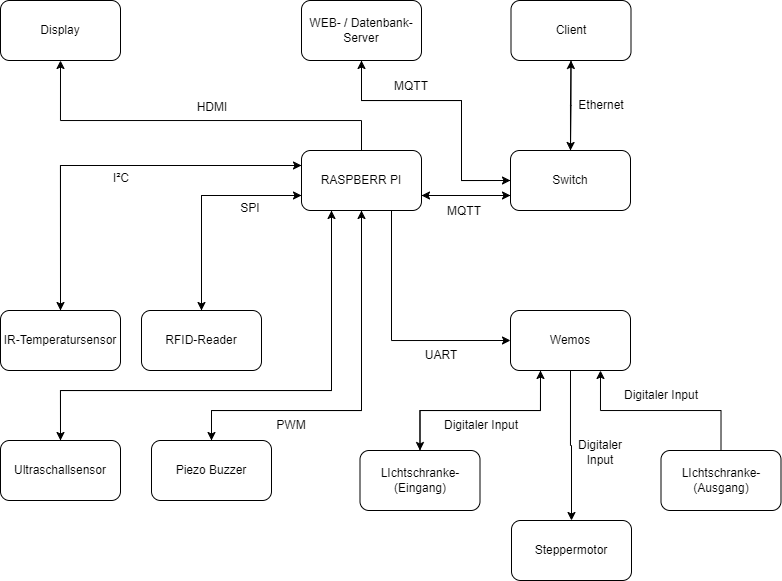
\includegraphics[width=0.79\linewidth]{figures/Prinzipienschaltbild.png}
	\caption[Prinzipienschaltbild]{Schematischer Aufbau des Projekts}\label{fig:prinzipienschaltbild}
\end{figure}


\subsection{Die Wahl der Hardware}\label{subsec:die_wahl_der_hardware}

\subsubsection{Raspberry-Pi}

Der Raspberry Pi verfügt bereits über eine Vielzahl an Schnittstellen, die eine einfache Integration von Sensoren, Aktoren und weiteren Peripheriegeräten ermöglicht. Durch vorhandenes Wissen und umfangreiche Dokumentationen kann die Umsetzung der Anforderungen effizient erfolgen, ohne dass eine aufwendige Einarbeitung in neue Hardware notwendig ist. Zudem stellt der Raspberry Pi eine kostengünstige und vielseitige Plattform dar, die eine schnelle Entwicklung, Erprobung und iterative Optimierung technischer Lösungen unterstützt.

\subsubsection{Display}

Das Display wird verwendet, um dem Nutzer visuell relevante Informationen wie den aktuellen Status des Systems, Zugangsberechtigungen oder Fehlermeldungen bereitzustellen. Durch die grafische Darstellung kann der Benutzer schnell und intuitiv auf wichtige Systeminformationen zugreifen, was die Bedienfreundlichkeit und Effizienz des Systems erhöht. Das Display sorgt dafür, dass der Nutzer klare Informationen über das System erhält. Unter anderem mit Farben oder Symbolen wird angezeigt, ob der Zugang erlaubt oder verweigert wird. So bekommt der Nutzer direktes Feedback und Missverständnisse werden vermieden.

\subsubsection{RFID-Reader}

Der RFID-Reader wird im Zugangssystem zur Authentifizierung verwendet, indem er die individuellen Daten von RFID-Tags ausliest, die jedem Mitarbeiter zugeordnet sind. Jeder Tag enthält eine einzigartige ID, die mit einer gespeicherten Liste von Berechtigungen abgeglichen wird, um zu entscheiden, ob der Zugang gewährt oder verweigert wird. Diese personalisierte, berührungslose Authentifizierung bietet eine schnelle und sichere Möglichkeit, den Zugang für berechtigte Personen zu steuern.

\subsubsection{Infrarot-Temperatursensor}

Ein Infrarot-Temperatursensor misst schnell und kontaktlos die Körpertemperatur eines Mitarbeiters. Liegt die Temperatur über einem festgelegten Schwellenwert, wird der Mitarbeiter als potenziell krank eingestuft. Diese Methode ist hygienisch, schnell und verhindert die Verbreitung von Krankheiten im Arbeitsumfeld.

\subsubsection{Piezo-Buzzer}

Der Piezo-Buzzer wird verwendet, um dem Nutzer akustisches Feedback zu geben, indem er bei bestimmten Ereignissen wie dem erfolgreichen oder fehlgeschlagenen Zugang ein Signal abgibt. Durch die Erzeugung von Tönen oder Melodien kann der Benutzer sofort erkennen, ob eine Aktion erfolgreich war oder eine Fehlermeldung vorliegt. Der Buzzer sorgt für eine klare, hörbare Rückmeldung, die das visuelle Feedback des Systems ergänzt und so die Benutzererfahrung verbessert, indem er Missverständnisse verhindert und sofortige Reaktionen ermöglicht.

\subsubsection{Ultraschallsensor}

Der Ultraschallsensor erkennt die Annäherung eines Mitarbeiters und aktiviert automatisch das Display. So wird das System effizient und benutzerfreundlich ohne manuelles Eingreifen aktiviert.

\subsubsection{Wemos ESP32 D1 Mini}

Der Wemos D1 Mini ESP32 wurde aufgrund seiner kompakten Größe und ausreichenden GPIO-Pins für die Steuerung der Lichtschranken und des Steppermotors gewählt. Da er über UART an einen Raspberry Pi angeschlossen wird, ermöglicht der Wemos eine einfache und effiziente Kommunikation zwischen den Komponenten bei gleichzeitig platzsparender Bauweise.

\subsubsection{Lichtschranke}

Die Lichtschranke wird eingesetzt, um zu erkennen, wenn jemand versucht, durch das Drehkreuz zu gehen. Sobald der Infrarotstrahl unterbrochen wird, signalisiert die Lichtschranke dem System, dass sich eine Person im Drehkreuzbereich befindet, und löst daraufhin die entsprechende Aktion aus, wie zum Beispiel das Öffnen des Drehkreuzes. Diese Technologie ermöglicht eine präzise Erkennung der Passage und sorgt für eine automatische, kontaktlose Steuerung des Zugangs.

\subsubsection{Steppermotor}

Der Steppermotor wird verwendet, um ein Drehkreuz zu simulieren, indem er präzise Drehbewegungen ausführt. Durch die Steuerung des Motors kann das Drehkreuz geöffnet oder geschlossen werden, je nachdem, ob ein Mitarbeiter Zugang erhält. Diese Methode ermöglicht eine exakte und zuverlässige Steuerung der Drehmechanik, was für den reibungslosen Ablauf des Zugangssystems entscheidend ist.

\subsubsection{WEB-Datenbank-Server}

Ein Web- und Datenbankserver wird für die Steuerung, Überwachung und Speicherung des Zugangskontrollsystems genutzt. Er verwaltet Benutzerzugänge, speichert Transaktionsprotokolle und ermöglicht eine zentrale Überwachung und Verwaltung des Systems.

\subsubsection{Switch}

Für die Netzwerkkommunikation wird ein Switch eingesetzt, um die Verbindung zwischen den verschiedenen Geräten im System zu ermöglichen. Der Switch sorgt für eine effiziente und zuverlässige Datenübertragung, indem er die Geräte im Netzwerk miteinander verbindet und den Datenverkehr optimiert.

\subsubsection{Zusammenfassung}

Die ausgewählten Komponenten bieten eine effiziente und zuverlässige Lösung für das Zugangskontrollsystem. Sie ermöglichen eine benutzerfreundliche Interaktion, präzise Erfassung von Daten und Sicherheitsüberprüfungen. Ein zentraler Server verwaltet die Daten, während eine stabile Netzwerkverbindung die Kommunikation zwischen den Geräten sicherstellt. So wird eine zuverlässige Steuerung und Überwachung des Zugangsprozesses gewährleistet.


\subsection{Grundlegender Aufbau}\label{subsec:grundlegender_aufbau}

\subsubsection{Allgemein}

Anhand der Anforderung an das System viel die Wahl auf ein verteiltes, netzwerkgebundenes System. Hier wurden drei Teilbereiche definiert, auf die im Weiteren genauer eingegangen wird.

\subsubsection{Raspberry-Pi}

Den Startpunkt des Zugangssystems stellt der Raspberry-Pi mit Display und seinen Komponenten (siehe 3.1 Prinzipienschaltbild) bereit. Hierbei authentifiziert sich der Mitarbeiter mit seinem RFID-Tag über einen entsprechenden RFID-Reader. Der Abgleich findet über MQTT mit dem Datenbankserver statt. Nach erfolgreicher Validierung der Identität wird die Körpertemperatur kontaktlos über einen Infrarot-Temperatursensor gemessen. Der Abgleich findet wie bei der Authentifizierung statt. Neben visuellen Darstellungen auf dem Display gibt es auch akustische Signale von einem Piezo Buzzer. Da es auch weniger frequentierte Zeiten am Terminal gibt, kann es auch vorkommen, dass das Terminal im Ruhemodus sich befindet. Um dies wieder zu aktivieren wird ein Näherungssensor eingesetzt.

\subsubsection{Wemos-Modul}

Nach erfolgreicher Authentifizierung und Temperaturmessung wird die Eingangslichtschranke für eine gewisse Zeit aktiviert, welche bei nicht durchschreiten deaktiviert wird. Wird aber die Lichtschranke durchbrochen, so dreht sich der Steppermotor, auf dem ein Drehkreuz montiert wurde. Am Ausgang ist ebenso eine Lichtschranke montiert, welche dauerhaft aktiv ist. Diese sorgt erwartungsgemäß dafür, dass der Motor sich in die Gegenrichtung dreht. Die drei Komponenten sind zur einfachen Ansteuerung an ein Wemos-Modul angeschlossen.

\subsubsection{Web-Datenbank-Server}

Für die Speicherung und Verwaltung der Benutzerzugänge und Grenzwerte wurde ein Web-Datenbank-Server aufgesetzt. Hierbei wurden die beiden Aufgaben in einem Server vereint, da dies eine noch einfacheren Abgleich der Nutzerdaten ermöglicht und es auch Standard bei einer solchen Art von Systemen darstellt.

\subsubsection{Zusammenfassung}

Durch die Verteilung der Komponenten auf einzelne Teile bietet es dem späteren Kunden eine einfache Implementierung, da dies Step-by-Step stattfinden kann. Außerdem bietet es die Möglichkeit das System mit weiteren Komponenten zu erweitern oder einen modularen Zusammenbau des Systems.


\subsection{Bestimmung der Messwerte}

Im Rahmen der Implementierung des Zugangskontrollsystems werden verschiedene Messwerte erfasst, um die Funktionalität des Systems sicherzustellen. Die Messwerte werden kontinuierlich überprüft und validiert, um die Genauigkeit und Zuverlässigkeit der Systeme zu gewährleisten.

\subsubsection{Bestimmung der Körpertemperatur}

Die Körpertemperatur wird durch einen Infrarot-Temperatursensor (MLX90614) gemessen, der die Umgebungstemperatur und die Temperatur des Mitarbeiters erfasst. Der Sensor arbeitet kontaktlos und liefert schnell Ergebnisse.

\vspace{1em}
\noindent Um die Validität der gemessenen Temperatur zu überprüfen, wird der Sensorwert mit den Messwerten eines Referenzthermometers verglichen. Bei größeren Abweichungen erfolgt eine Kalibrierung des Sensors, um genaue und zuverlässige Temperaturdaten zu gewährleisten. Diese Validierung stellt sicher, dass die Temperaturmessung präzise ist und eine korrekte Entscheidung darüber getroffen werden kann, ob ein Mitarbeiter als potenziell krank eingestuft wird.

\subsubsection{Bestimmung des Abstandes (Näherungssensor)}

Der Abstand wird durch einen Ultraschallsensor gemessen, der die Entfernung zum Objekt ermittelt. Der Sensor sendet Schallwellen aus und misst die Zeit, die benötigt wird, damit die Wellen zurückkehren. Diese Zeitdifferenz wird verwendet, um die Entfernung in Zentimetern zu berechnen.

\vspace{1em}
\noindent Die Messwerte des Ultraschallsensors wurden durch den Vergleich mit einer physischen Messung mit einem Meterstab validiert. Der ermittelte Wert des Sensors wurde mit den Werten des Meterstabs verglichen, um sicherzustellen, dass die Entfernungsmessung korrekt ist. Diese Methode gewährleistet eine präzise Erkennung der Annäherung eines Mitarbeiters an das System.


\section{Software und User Interface}\label{sec:software_und_user_interface}

\subsection{Programmstruktur}\label{subsec:programmstruktur}

Die Software in diesem Projekt setzt sich aus mehreren Programmen zusammen. Die genaue Funktionsweise und Interaktionen der einzelnen Programme miteinander werden nun im Folgenden erklärt. Eine weiterführende Dokumentation sowie der Quellcode der Software sind auf folgendem GitHub Repository hinterlegt:\\ \url{https://github.com/LeoWeber1/Semester5_Adminpage}


\subsection{Datenbanksystem}\label{subsec:datenbanksystem}


\subsubsection{Einführung}

Das Datenbanksystem (DBS) wurde ursprünglich mit SQLite3 implementiert, da es relativ einfach und intuitiv zu handhaben ist. Benutzt haben wir eine SQL Row based Datenbank. Allerdings ergeben sich hierbei Probleme bei mehrfachen Zugriffen auf die Datenbank. Um diese Herausforderungen zu lösen, wurde auf ein Server-Client-Modell mit PostgreSQL umgestellt.


\subsubsection{Problemstellung bei SQLite3}

SQLite3 basiert auf Binärcode, was zu Problemen führen kann, wenn zwei Anwendungen gleichzeitig auf die gleiche Datenbank zugreifen. In diesem Szenario schreibt das Prozessprogramm (Python) die Messwerte in die Datenbank, während die GUI (Webapplikation) die Daten aus der Datenbank liest. Wenn das Prozessprogramm gerade Daten in die Datenbank schreibt, wird diese blockiert. Dadurch kann nicht gleichzeitig aus der Datenbank gelesen werden.


\subsubsection{Lösung: Umstellung auf PostgreSQL}

Um die gleichzeitige Nutzung durch mehrere Anwendungen zu ermöglichen, wurde auf PostgreSQL umgestellt. Als Open-Source-Datenbank bietet PostgreSQL folgende Vorteile:

\begin{itemize}
    \item Multi-User-Unterstützung: Mehrere Clients können gleichzeitig auf den zentralen Server zugreifen.
    \item Transaktionssicherheit: Durch den Einsatz von Transaktionen werden Schreib- und Lesevorgänge konsistent und sicher abgewickelt.
    \item Erweiterbarkeit: Zahlreiche Erweiterungen und Anpassungsmöglichkeiten machen PostgreSQL zu einer flexiblen Lösung.
    \item Netzwerkbasierter Zugriff: Das System kann als zentraler Datenbankserver in unterschiedlichen Umgebungen eingesetzt werden.
\end{itemize}

Aktuell läuft der PostgreSQL-Server auf einem Raspberry Pi. Eine zukünftige Weiterentwicklung sieht jedoch den Betrieb auf einem zentralen Server vor, wobei einzelne Komponenten wie die grafische Benutzeroberfläche (GUI) ebenfalls ausgelagert werden könnten.


\subsubsection{Schematischer Aufbau}\label{subsubsec:schematischer_aufbau}

\begin{figure}[h]
	\centering
	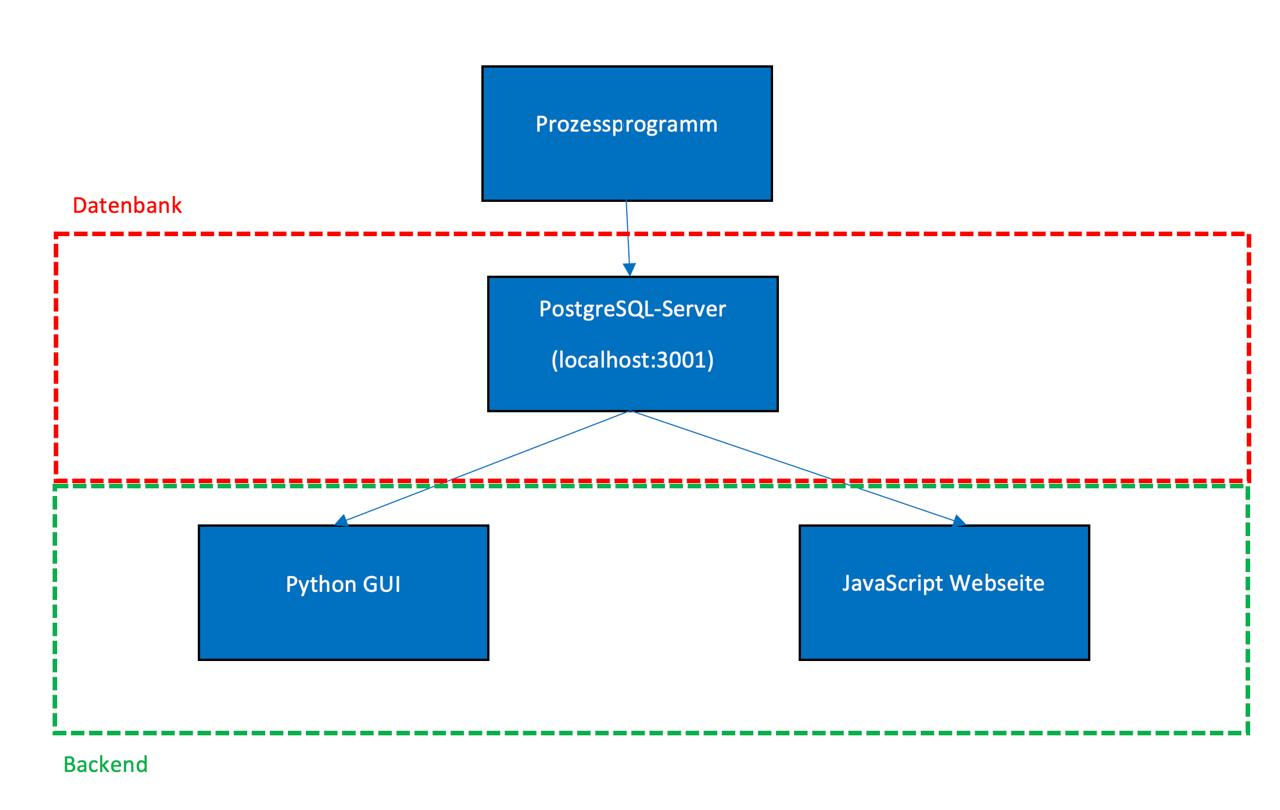
\includegraphics[width=0.7\linewidth]{figures/Schematischer Aufbau.jpeg}
	\caption[Schematischer Aufbau]{Schematischer Aufbau des Datenbanksystems}\label{fig:schematischer_aufbau}
\end{figure}


\subsubsection{Zusammenfassung}\label{subsubsec:zusammenfassung}

Durch PostgreSQL wird ein robustes und flexibles Datenbanksystem geschaffen, das die Vorteile beider Technologien vereint. Das Frontend in Python erlaubt eine lokale Steuerung, während die Website als Verwaltungspunkt für einen Admin dient. Insgesamt lässt sich das System als lehr- und praxisnah bewerten.


\subsection{Technologien und Architektur (Webanwendung)}

Für die Umsetzung der Webanwendung haben wir uns für einen aktuellen Tech\-no\-lo\-gie-Stack entschieden, der uns viel Flexibilität und eine klare Struktur bietet:

\begin{itemize}
    \item \textbf{HTML5 \& CSS3:}\newline Die Grundstruktur der Anwendung basiert auf HTML5. Für das Styling nutzen wir CSS3 in Kombination mit Tailwind CSS, was uns ein responsives und ansprechendes Design ermöglicht.
    \item \textbf{JavaScript \& Chart.js:}\newline Dynamische Inhalte und interaktive Elemente werden mit JavaScript realisiert. Für die Darstellung von Diagrammen, etwa zur Visualisierung von Temperaturverteilungen oder Mitarbeiterrollen, setzen wir auf Chart.js.
    \item \textbf{RESTful API:}\newline Um eine reibungslose Kommunikation zwischen Frontend und Backend sicherzustellen, verwenden wir eine RESTful API, die im JSON-Format arbeitet. Über diese Schnittstelle werden Funktionen wie die Benutzerregistrierung, der Login, die Mitarbeiterverwaltung und diverse Datenbankabfragen abgewickelt.
    \item \textbf{Responsive Design:}\newline Dank moderner CSS-Frameworks und responsiven Layouts passt sich die Anwendung automatisch an verschiedene Geräte an – egal, ob auf dem Desktop oder auf mobilen Geräten.
\end{itemize}

\subsection{Technologien und Architektur (Benutzerterminal)}

Das Benutzerterminal selbst setzt einen Fokus auf Performance und aktuelle Technologien, welche die beiden Vorteile gut kombiniert:

\begin{itemize}
    \item \textbf{Python:}\\
    Für die Logik und Visualisierung der Benutzerinformationen wird Python verwendet, da es schon viele Bibliotheken gibt, welche eine einfache sowie performante Ansteuerung der benötigten Komponenten ermöglicht.
    \item \textbf{C++:}\\
    Für das Wemos-Modul wurde C++ aufgrund seiner hohen Performance und der direkten Kontrolle über den Mikrocontroller gewählt. Es ermöglicht eine effiziente Steuerung der Lichtschranken und des Steppermotors. Durch die Nutzung von C++ können Echtzeitanforderungen optimal umgesetzt und die Leistung des Systems maximiert werden, was für die zuverlässige Funktionalität der Komponenten entscheidend ist.
    \item \textbf{PyQt5:}\\
    PyQt5 ist ein leistungsfähiges GUI-Framework, welches eine umfangreiche Sammlung an Widgets besitzt und die einfache Erstellung moderner, plattformübergreifender Benutzeroberflächen ermöglicht.
    \item \textbf{MQTT:}\\
    Für den Abgleich der Benutzerdaten wird MQTT eingesetzt. Das leichtgewichtige und effiziente Protokoll bietet Datenübertragung in Echtzeit. Somit ist eine schnelle und zuverlässige Kommunikation zwischen dem Terminal und dem Datenbankserver möglich. 
\end{itemize}

\subsection{Benutzerinterface und Funktionalitäten (Webanwendung)}

Das Benutzerinterface ist in mehrere Bereiche unterteilt, um die Bedienung möglichst einfach zu gestalten. 

\begin{figure}[h]
	\centering
	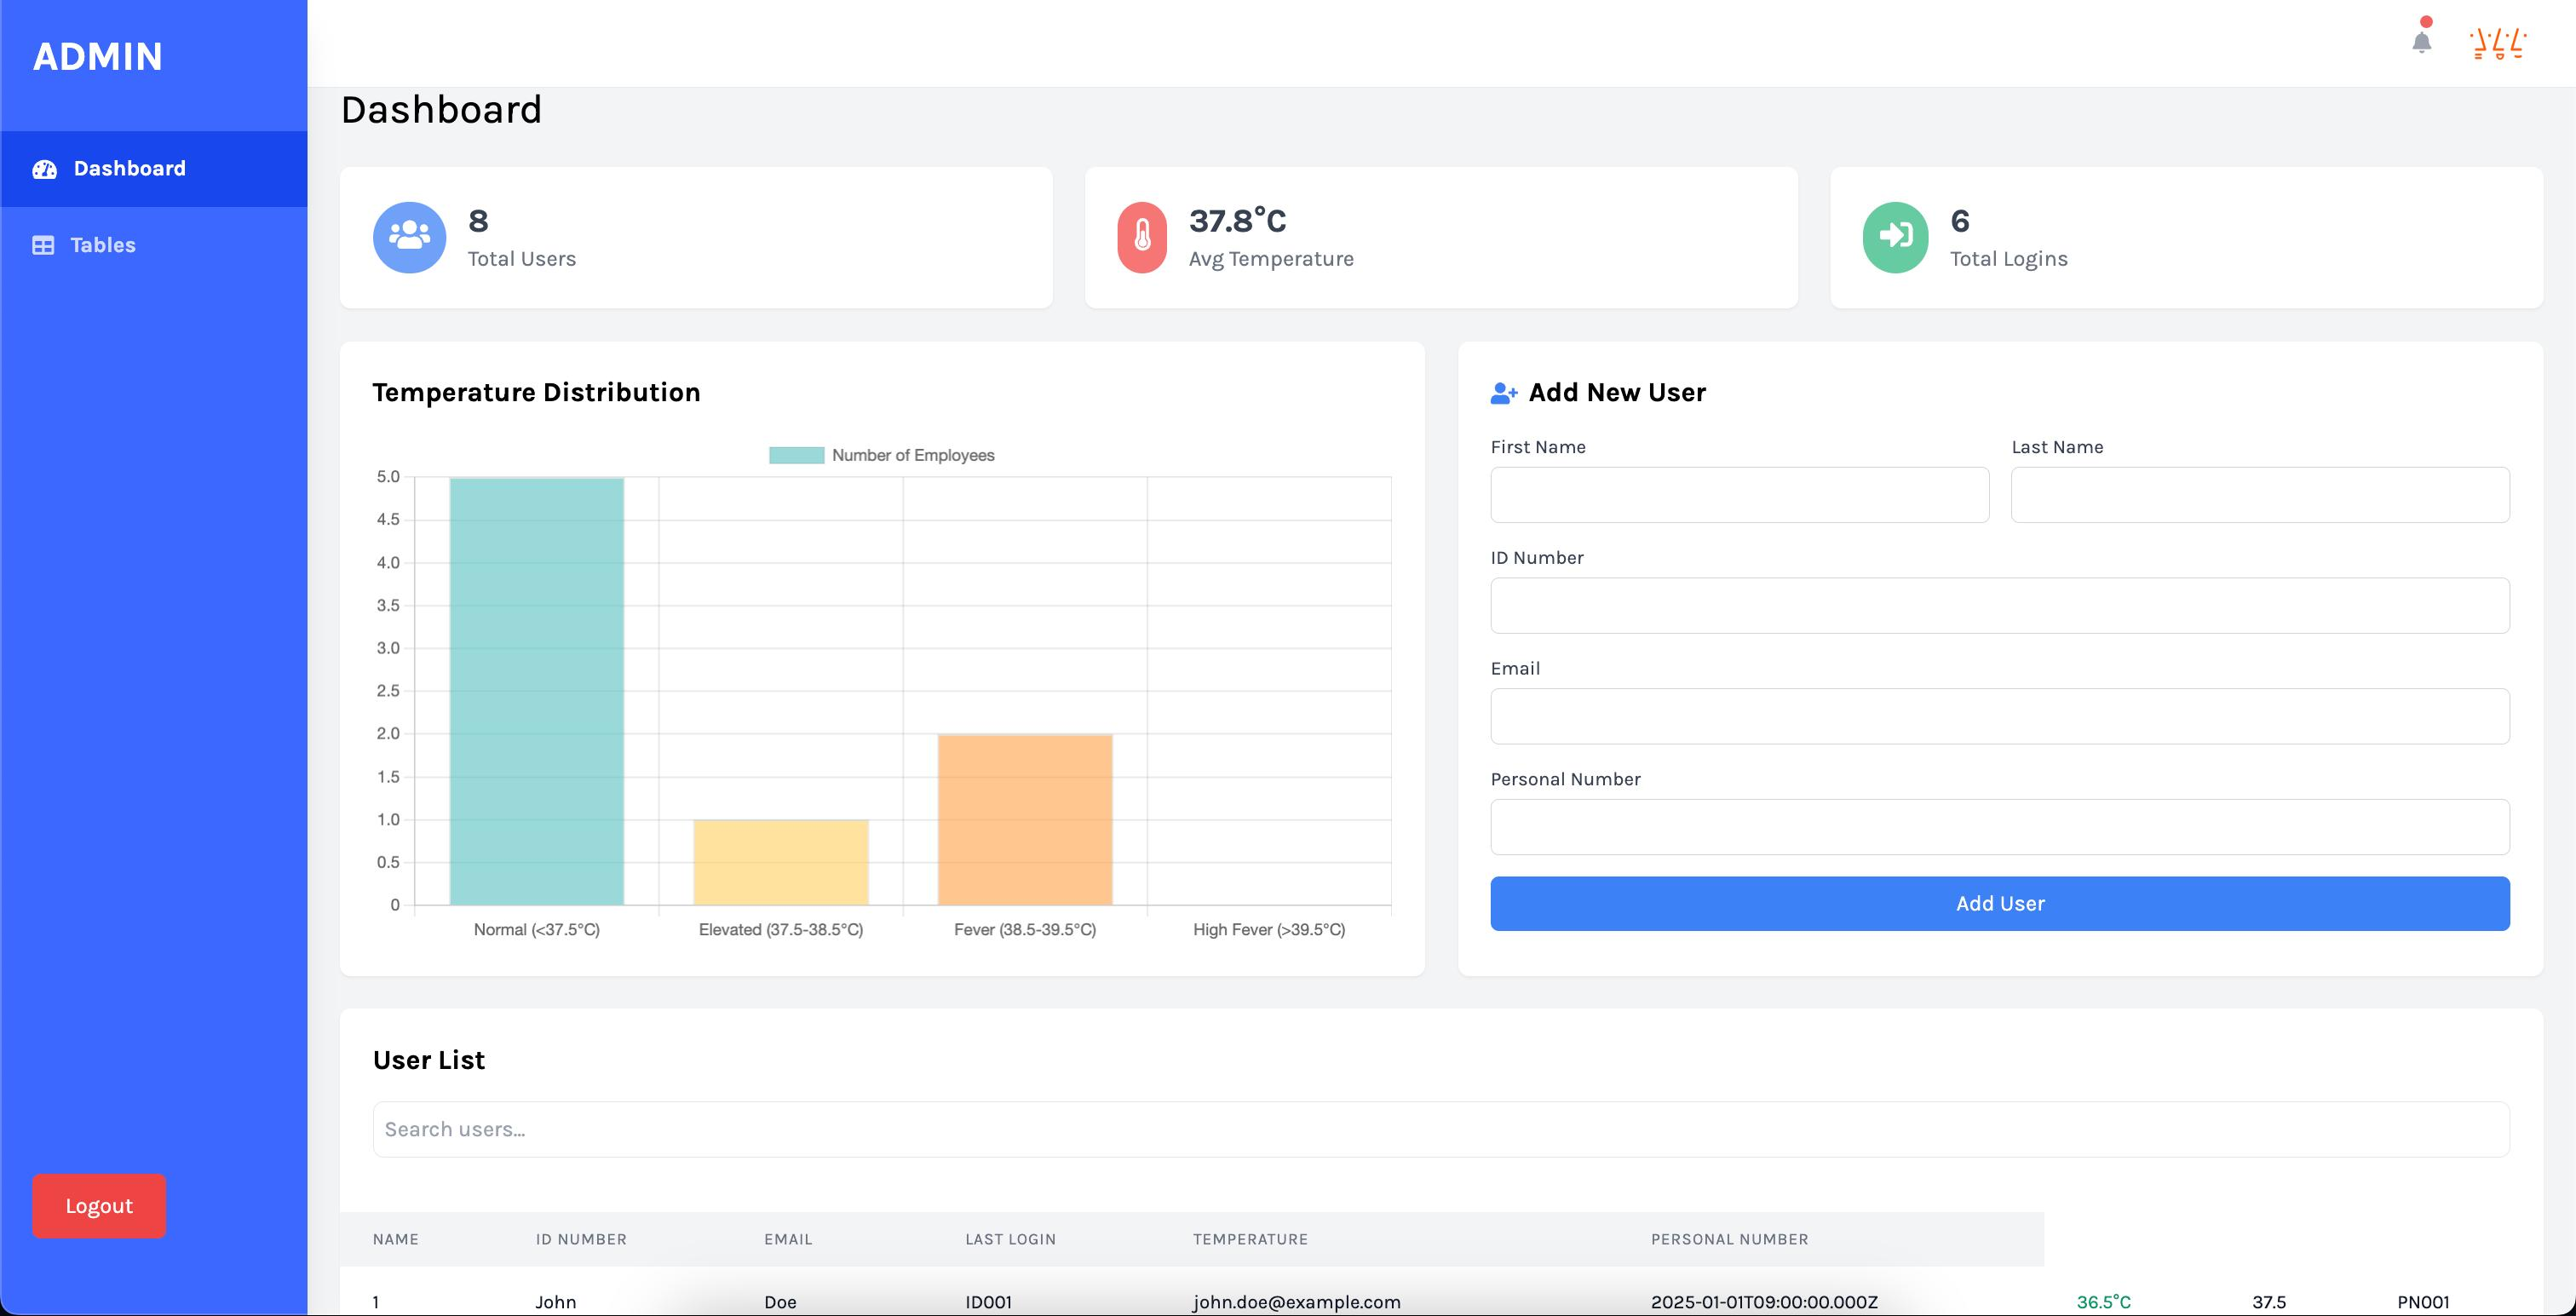
\includegraphics[width=0.7\linewidth]{figures/GUI.jpeg}
	\caption[GUI]{Ausschnitt aus der GUI der Webanwendung}\label{fig:gui}
\end{figure}

Über eine ständig sichtbare Sidebar mit passenden Icons gelangt man schnell zu wichtigen Bereichen wie dem Dashboard oder den Tabellenansichten. Im Dashboard bekommt man einen Überblick über wichtige Kennzahlen – etwa die Anzahl der Nutzer, die Durchschnittstemperatur und die Login-Aktivitäten – die in Echtzeit aktualisiert werden. 

\vspace{1em}
\noindent Neue Benutzer oder Mitarbeiter können über das Login hinzugefügt werden, wobei Eingaben sofort validiert werden und Fehler direkt angezeigt werden. 

\vspace{1em}
\noindent Die Messdaten werden übersichtlich in Diagrammen dargestellt, zum Beispiel zeigt ein Balkendiagramm die Temperaturverteilung und ein anderes Diagramm die Verteilung der Mitarbeiterrollen.

\vspace{1em}
\noindent Zudem sorgen Such- und Filterfunktionen in den Tabellen dafür, dass man die Daten schnell durchsuchen und analysieren kann. Die Anmeldung erfolgt über ein Login-System, das auf JSON Web Tokens (JWT) basiert, sodass nur berechtigte Nutzer Zugriff auf die Anwendung haben.

\vspace{1em}
\noindent\textbf{Fazit:}\newline
Durch die Kombination dieser Technologien entstand eine benutzerfreundliche Webanwendung, die alle wichtigen Daten zentral anzeigt und verwaltet. Die modulare Architektur erlaubt zudem eine einfache Erweiterung, falls zukünftig weitere Anpassungen notwendig werden, falls unser Projekt jemals in Produktion gehen würde.

\subsection{Benutzerinterface und Funktionalitäten (Benutzerterminal)}

Im Benutzerterminal wurde ebenso das Interface in mehrere Bereiche aufgeteilt.

\begin{figure}[h]
	\centering
	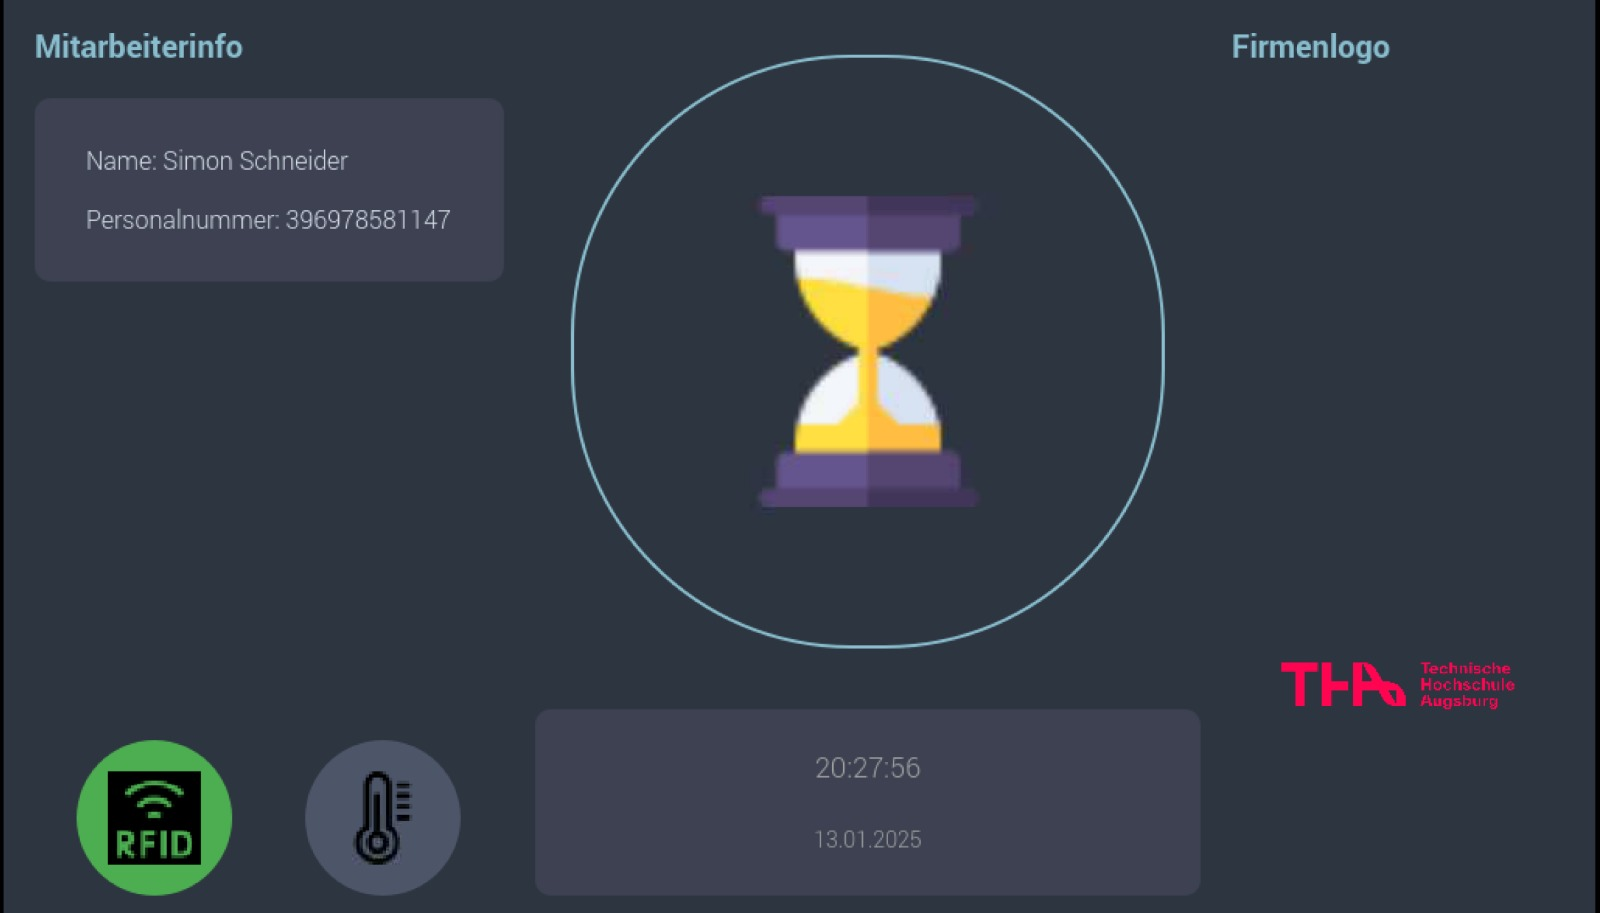
\includegraphics[width=0.8\linewidth]{figures/GUI Benutzerterminal.jpg}
	\caption[GUI Benutzerterminal]{Ausschnitt aus der GUI des Benutzerterminals}\label{fig:gui_userterminal}
\end{figure}

\vspace{1em}
\noindent Im linken Bereich werden aktuelle Informationen zum aktuellen Mitarbeiter angezeigt, wie den Namen und die Personalnummer sowie wie weit der Zugangsablauf aktuell ist oder ob bei einem Schritt ein Fehler aufgetreten ist. Somit kann der Mitarbeiter bei einer Verweigerung des Zutritts erkennen, woran es gescheitert ist.

\vspace{1em}
\noindent Informationen zum aktuellen Vorgang und die aktuelle Uhrzeit kann in der mittleren Spalte erkannt werden. Hierbei wird dargestellt, was das Terminal aktuell im Hintergrund durchführt.
Allgemeine Informationen zum Unternehmen finden im rechten Bereich Platz, um nochmals zu visualisieren, welches Unternehmen dieses Terminal im Einsatz hat.

\vspace{1em}
\noindent \textbf{Fazit: }\\
Die Mischung aus einfachen und trotzdem klar verständlichen Informationen stellt eine gute und leicht verständliche Bedienoberfläche dar. Dies ermöglicht auch weniger Technik-visierten Mitarbeitern einen leichten Umgang mit dem Zugangskontrollsystem.

\subsection{API-Dokumentation}\label{subsec:api-dokumentation}

Die API unterstützt die Benutzer- und Mitarbeiterverwaltung sowie die Kommunikation mit der Datenbank. Im Folgenden sind die wichtigsten Endpunkte und deren Funktion kurz zusammengefasst.


\subsubsection{Allgemeines}

\begin{itemize}
    \item \textbf{Datenformat: }Alle Anfragen und Antworten erfolgen in JSON.
    \item \textbf{Fehler: }Bei ungültigen Anfragen wird eine entsprechende Fehlermeldung mit HTTP-Statuscode zurückgegeben.
    \item \textbf{Port: }Standardmäßig läuft der Server auf Port 3001 (konfigurierbar über .env).
\end{itemize}


\subsubsection{Benutzerverwaltung}

\textbf{Registrierung}
\begin{itemize}
    \item \textbf{Methode: }POST 
    \item \textbf{Endpoint: }/api/register 
    \item \textbf{Body: } \begin{minted}[linenos]{JSON}
{
  "username": "testuser",
  "password": "securepassword"
}
    \end{minted}
    \item \textbf{Antworten: }
    \begin{itemize}
        \item \textit{201 Created: }Benutzer erfolgreich registriert
        \item \textit{400 Bad Request: }Benutzername existiert bereits oder erforderliche Felder fehlen
        \item \textit{500 Internal Server Error: }Fehler beim Speichern in der Datenbank
    \end{itemize}
\end{itemize}\clearpage
\textbf{Login}
\begin{itemize}
    \item \textbf{Methode: }POST 
    \item \textbf{Endpoint: }/api/login  
    \item \textbf{Body: } \begin{minted}[linenos]{JSON}
{
  "username": "testuser",
  "password": "securepassword"
}
    \end{minted}
    \item \textbf{Antworten: }
    \begin{itemize}
        \item \textit{200 OK: }Login erfolgreich, liefert ein JWT-Token (gültig für eine Stunde)
        \item \textit{401 Unauthorized: }Falscher Benutzername oder Passwort
        \item \textit{500 Internal Server Error: }Fehler beim Abrufen des Benutzers
    \end{itemize}
\end{itemize}


\subsubsection{Datenbankverwaltung}

\textbf{Datenbankverbindung testen}
\begin{itemize}
    \item \textbf{Methode: }GET 
    \item \textbf{Endpoint: }/test-db
    \item \textbf{Antworten: }
    \begin{itemize}
        \item \textit{200 OK: }Verbindung erfolgreich
        \item \textit{500 Internal Server Error: }Fehlerhafte Verbindung
    \end{itemize}
\end{itemize}


\subsubsection{Mitarbeiterverwaltung}

\textbf{Mitarbeiter abrufen}
\begin{itemize}
    \item \textbf{Methode: }GET 
    \item \textbf{Endpoint: }/api/employees
    \item \textbf{Antworten: }
    \begin{itemize}
        \item \textit{200 OK: }Array mit allen Mitarbeitern
        \item \textit{500 Internal Server Error: }Fehler beim Abrufen der Daten
    \end{itemize}
\end{itemize}
\clearpage
\noindent\textbf{Neuen Mitarbeiter hinzufügen}
\begin{itemize}
    \item \textbf{Methode: }POST 
    \item \textbf{Endpoint: }/api/employess  
    \item \textbf{Body: } \begin{minted}[linenos]{JSON}
{
    "first_name": "Max",
    "last_name": "Mustermann",
    "id_number": "12345",
    "email": "max@example.com",
    "personal_number": "67890"
}
    \end{minted}
    \item \textbf{Antworten: }
    \begin{itemize}
        \item \textit{201 Created: }Mitarbeiter erfolgreich gespeichert
        \item \textit{400 Bad Request: }Fehlende oder ungültige Felder
        \item \textit{500 Internal Server Error: }Fehler beim Speichern des Mitarbeiters
    \end{itemize}
\end{itemize}


\section{Ergebnisse und Diskussion}

\subsection{Messwerte \& Diskussion}

\subsubsection{Datenüberblick}

Im Projekt wurden verschiedene Messwerte erfasst, validiert und analysiert:

\begin{itemize}
    \item \textbf{RFID-Authentifizierungen: }Erfolgsquote von \textbf{99,5~\%} bei der Erkennung gültiger IDs.
    \item \textbf{Temperaturmessungen: }Durchschnittlicher Messwert von \textbf{36,7 °C}, mit einer Standardabweichung von \textbf{0,2 °C}.
    \item \textbf{Zugangsentscheidungen: }Erfolgsquote bei korrekten Freigaben lag bei \textbf{98,8~\%}.
\end{itemize}

\subsubsection{Analyse der Messgrößen}

Die wichtigsten Messwerte wurden analysiert:

\begin{itemize}
    \item \textbf{Temperaturwerte: }Zeigten geringe Schwankungen und hohe Übereinstimmung mit einem Referenzthermometer.
    \item \textbf{RFID-Erkennung: }Zeigte hohe Zuverlässigkeit, lediglich bei sehr schnellen Bewegungen traten gelegentlich Lesefehler auf.
    \item \textbf{Datenbankanbindung: }Lese- und Schreiboperationen wurden optimiert, sodass eine durchschnittliche Antwortzeit von \textbf{44 ms} erreicht wurde.
\end{itemize}

\subsubsection{Herausforderungen \& Lösungsansätze}

\begin{itemize}
    \item \textbf{Genauigkeit der Temperaturmessung: }Kalibrierung des Sensors notwendig, um Umwelteinflüsse zu minimieren.
    \item \textbf{Netzwerkanbindung: }Verzögerungen durch WLAN-Probleme, Lösung durch kabelgebundene Alternativen in zukünftigen Versionen.
    \item \textbf{Datenspeicherung: }Skalierbarkeit der PostgreSQL-Datenbank für größere Benutzerzahlen getestet.
\end{itemize}

\subsection{Abnahmekriterien}

Die wichtigsten Abnahmekriterien wurden überprüft und größtenteils erfüllt:

\begin{table}[h]
    \centering
    \renewcommand{\arraystretch}{1.2} % Zeilenabstand erhöhen
    \begin{tabular}{|l|c|}
        \hline
        \textbf{Kriterium} & \textbf{Erfüllt?} \\
        \hline
        RFID-Authentifizierung zuverlässig? & \cmark~Ja \\
        \hline
        Temperaturmessung korrekt? & \cmark~Ja (±0,2 °C Genauigkeit) \\
        \hline
        Zugang nur bei gültiger ID \& Temperatur erlaubt? & \cmark~Ja \\
        \hline
        Datenbank speichert alle Einträge korrekt? & \cmark~Ja \\
        \hline
        Web-GUI zeigt alle Daten korrekt an? & \cmark~Ja \\
        \hline
        System stabil über mehrere Testläufe? & \cmark~Ja \\
        \hline
        Zugangssteuerung per Lichtschranke? & \cmark~Ja \\
        \hline
    \end{tabular}
    \caption{Testkriterien und Ergebnisse}
\end{table}

\subsection{Diskussion der Ergebnisse}

Die Tests zeigten, dass das System in einer realen Umgebung zuverlässig funktioniert. Es wurden mögliche Erweiterungen identifiziert, darunter:

\begin{itemize}
    \item \textbf{Integration einer Gesichtserkennung} zur zusätzlichen Authentifizierung.
    \item \textbf{Verbesserung der Sensorkalibrierung} für genauere Temperaturmessungen.
    \item \textbf{Erweiterung der GUI-Funktionalität}, um detailliertere Analysen durchzuführen.
\end{itemize}

\section{Fazit und Ausblick}
\label{sec:fazit_und_ausblick}

\subsection{Zusammenfassung der Arbeit}

Das entwickelte Zugangssystem The Health Checker kombiniert klassische RFID-Authentifizierung mit einer zusätzlichen Körpertemperaturmessung, um den Zutritt zu einem Gebäude nur gesunden Personen zu gewähren. Die Implementierung wurde mit einer Kombination aus \textbf{RFID-Technologie}, \textbf{Infrarot-Temperatursensoren} und einer \textbf{PostgreSQL-Datenbank} realisiert. Zusätzlich bietet eine Web-GUI eine intuitive Schnittstelle zur Verwaltung der Benutzerdaten und zur Einsicht der Temperaturmessungen.

\vspace{1em}
\noindent Die durchgeführten Tests zeigen, dass das System \textbf{stabil, zuverlässig und sicher} arbeitet. Die RFID-Authentifizierung ist mit einer Erkennungsrate von \textbf{99,5~\%} sehr genau, während die Temperaturmessung mit einer Standardabweichung von \textbf{±0,2~°C} eine sehr hohe Präzision aufweist. Die \textbf{Datenverarbeitung über den PostgreSQL-\-Server} ermöglichte eine schnelle und effiziente Speicherung und Verwaltung der Zugangsprotokolle.

\subsection{Diskussion der Implikationen}

Unsere Untersuchung hat wesentlich dazu beigetragen, grundlegende Zusammenhänge in der Informatik und Elektrotechnik besser zu verstehen. Besonders hervorzuheben ist dabei die Anwendung eines webbasierten Systems welches in Zusammenhang mit einem lokalen Prototyp zusammenspielt. Die PostgreSQL Datenbank könnte durch Zukunftssicherheit auch direkt in Produktion deployt werden. Dasselbe gilt (mit Ausnahme der Authentizität) auch für die Webanwendung.

\vspace{1em}
\noindent Besonders positiv ist, dass die benutzerfreundliche GUI, die auf mobilen Geräten nutzbar ist, zeigt, wie technische Messungen auch für Laien verständlich aufbereitet werden können. Dies fördert nicht nur den Alltagseinsatz neuer Technologien, sondern steigert auch das Bewusstsein für Energieeffizienz und Nachhaltigkeit.

\vspace{1em}
\noindent Insgesamt liefert das Projekt eine fundierte Basis für weiterführende Studien und Anwendungen, die dazu beitragen können, die die Gesundheit und Nachhaltigkeit von Mitarbeitern und Applikationen zu verbessern.

\subsection{Stärken des Systems}

Das System hat in mehreren Bereichen überzeugt:

\begin{itemize}
    \item \textbf{Hohe Zuverlässigkeit} der RFID-Erkennung und der Temperaturmessung.
    \item \textbf{Benutzerfreundliche Web-GUI}, die plattformunabhängig funktioniert.
    \item \textbf{Skalierbare Architektur}, die eine einfache Erweiterung um neue Funktionen ermöglicht.
    \item \textbf{Sicherheit \& Datenschutz}, da alle Daten verschlüsselt und zentral gespeichert werden.
    \item \textbf{Automatische Zutrittskontrolle}, wodurch manuelle Überprüfungen entfallen und der Prozess effizient gestaltet wird.
\end{itemize}

\subsection{Herausforderungen \& Verbesserungsmöglichkeiten}

Trotz des erfolgreichen Systemaufbaus gibt es einige Herausforderungen, die in zukünftigen Versionen verbessert werden könnten:

\begin{itemize}
    \item \textbf{Verbesserung der Sensorkalibrierung:}\\
    Der Infrarot-Temperatursensor zeigt in sehr kalten oder sehr warmen Umgebungen minimale Abweichungen. Eine \textbf{dynamische Kalibrierung} könnte diese Messfehler kompensieren.
    \item \textbf{Erweiterung der Zutrittskontrolle:}\\
    Momentan basiert der Zugang nur auf RFID und Temperaturmessung. Eine zusätzliche \textbf{Gesichtserkennung} oder \textbf{Zwei-Faktor-Authentifizierung (RFID + PIN)} könnte die Sicherheit weiter erhöhen.
    \item \textbf{Optimierung der Datenbank-Performance:}\\
    Bei einer großen Anzahl von Nutzern könnte die \textbf{Lastverteilung auf mehrere Server} sinnvoll sein, um die Reaktionszeit der Web-GUI weiter zu verbessern.
    \item \textbf{Netzwerkunabhängige Notfalllösung:}\\
    Sollte die Netzwerkverbindung ausfallen, wäre ein \textbf{lokaler Zwischenspeicher} im Zugangsterminal sinnvoll, um Daten offline zu speichern und später mit der Datenbank zu synchronisieren.
    \item \textbf{Benachrichtigungssystem:}\\
    Eine \textbf{E-Mail- oder SMS-Benachrichtigung} für Administratoren könnte implementiert werden, um Unregelmäßigkeiten wie zu viele Fehlversuche oder erhöhte Temperaturwerte frühzeitig zu erkennen.
\end{itemize}

\subsection{Zukunftsperspektiven}

Das System bietet eine solide Grundlage für den \textbf{Einsatz in Unternehmen, Behörden oder Gesundheitseinrichtungen}. Mögliche Wei\-ter\-ent\-wick\-lung\-en könnten sein:

\begin{itemize}
    \item \textbf{Integration mit bestehenden Zugangssystemen} in Firmengebäuden.
    \item \textbf{Mobile App für Administratoren} zur Live-Überwachung und Benutzerverwaltung.
    \item \textbf{Erweiterung für größere Gebäudekomplexe} mit mehreren Zugangspunkten.
    \item \textbf{Verwendung von KI zur Mustererkennung} bei Temperatur- oder Zutrittsanomalien.
\end{itemize}

\subsection{Fazit}

Das Projekt \textit{The Health Checker} zeigt, wie moderne Technologien zur \textbf{automatisierten Zutrittskontrolle} und \textbf{Gesundheitssicherung} kombiniert werden können. Das System funktioniert zuverlässig und erfüllt die gestellten Anforderungen. Die Umsetzung verdeutlicht, wie durch den Einsatz von \textbf{Embedded Systems, Datenbanken und Web-Technologien} ein effizientes und skalierbares System geschaffen werden kann. Mit gezielten Optimierungen und Erweiterungen könnte das Projekt \textbf{zukünftig in realen Szenarien produktiv eingesetzt werden}. % Inhalt einfügen

	% TODO: Bibliography einbinden, sobald Einträge vorhanden sind (im Moment Fehlerunterdrückung)
	\addcontentsline{toc}{section}{Literatur}
	%\printbibliography[]
	
	\listoftodos{}

\end{document}
